% ch-wetting.tex -- theory: disjoining pressure, contact angle, equilibrium drops, sizing
\chapter{濡れと接触線}
\label{ch:wetting}

長波長近似は勾配が小さいことを前提とする。しかし接触線の近くでは、液膜の中で唯一、勾配が小さくない。
Yuzenは、潤滑近似モデルで一般的な方法でこれに対処する。膜厚がゼロにならないようにし、いたるところに
薄い前駆膜を残す。そのうえで分離圧を加え、前駆膜から液滴への遷移部分で正しい平衡接触角が再現されるように
する。

この方法は有効だが、適用できる範囲には定量的な限界がある。本章では、まず較正を導出し、解析的に確認した
うえで、平衡液滴を解く。次に、指定した接触角がケースで実現できるかどうかを左右する二つの要因を示す。
前駆膜に対する液滴の厚さと、遷移領域に対する格子の細かさである。濡れの計算を設定する場合、入力ファイルの
書き方に直接かかわるのは最後の二節である。

\section{分離圧モデルと\texorpdfstring{$\Dpn$}{Dp}の較正}
\label{sec:wetting:dp}

有次元の形で書くと、分離圧は

\begin{equation}\label{eq:pi-dim}
  \Pi(h) = B \left[ (\hstar/h)^{n} - (\hstar/h)^{m} \right],
  \qquad n > m > 1,
\end{equation}

である。$\hstar$は前駆膜の厚さであり、指数の組には慣例的に$(n,m) = (3,2)$を用いる。
第一項は斥力、第二項は引力を表し、両者は$h = \hstar$でちょうど釣り合う。この組は
\key{ExponentN}と\key{ExponentM}の既定値である。\key{Physics.DisjoiningPressure}ブロックに
これらを書かなかった場合も、ブロックごと省いた場合も、この値になる（\cref{tab:physics-disjoining-keys}）。

係数$B$は任意に選べるわけではない。モデルが指定の平衡接触角$\thetae$を再現するという条件から決まる。
この条件はエネルギー収支であり、\emph{濡れた基板と乾いた基板の表面エネルギーの差が、膜厚方向の分離圧の
積分に等しい}ことを表す。式で書くと

\begin{equation}\label{eq:energy-balance}
  \sigma\,(1 - \cos\thetae)
    = \frac{B\,\hstar\,(n-m)}{(n-1)(m-1)},
\end{equation}

となり、これを$B$について解くと

\begin{equation}\label{eq:B-coef}
  B = \frac{(n-1)(m-1)}{\hstar\,(n-m)}\,\sigma\,(1 - \cos\thetae).
\end{equation}

を得る。長波長の領域では$\thetae$は小さいので、$1-\cos\thetae$を$\thetae^{2}/2$で置き換える。
この近似の誤差は\cref{tab:cos-error}に厳密な値で示しており、指定する角度を小さく保つべき理由の
一つでもある。\cref{eq:B-coef}を圧力スケール$\sigma h_0 / L_0^{2}$で割ると、コードで実際に
用いる係数が得られる。

\begin{equation}\label{eq:dp-def}
  \Dpn = \frac{\As\,(n-1)(m-1)}{2\,\Hstar\,(n-m)}\;\thetae^{2}.
\end{equation}

\cref{eq:dp-def}からは、どの設定が何に効くかが明らかになる。角度\key{ContactAngle}は
$\Dpn$を$\thetae^{2}$に比例して変えるので、濡れの挙動を決めるキーになる。他の三つ、つまり
\key{ExponentN}、\key{ExponentM}、前駆膜の比$\Hstar$も\cref{eq:dp-def}に現れる。これは、
角度に対するこれらの効果を打ち消すためである。

\begin{note}[指数や前駆膜の比を変えても目標の角度は変わらない]
  $\Dpn$は毎回$n$、$m$、$\Hstar$から計算し直す。そのため、これらをどう変えても、モデルが目指す角度は
  $\thetae$のままである。変わるのは、前駆膜の厚さと、前駆膜から液滴への遷移領域の幅である。
  その結果、\cref{sec:wetting:apparent,sec:wetting:sizing}に示すように、指定した角度がどこまで
  実現されるか、またそれを捉えるのにどれだけ細かい格子が必要かが変わる。
\end{note}

\section{解析的な確認}
\label{sec:wetting:analytic}

\cref{eq:dp-def}が接触角と整合することは、数値計算をせずに厳密に確認できる。
前駆膜が無限遠まで続く極限、すなわち圧力ゼロ（$K = 0$）で遠方の膜厚が$\Hf = \Hstar$の場合を考える。
液膜全体にわたる無次元分離圧の積分は、初等的に求まる。

\begin{equation}\label{eq:pi-integral}
  \int_{\Hstar}^{\infty} \Pihat\,\mathrm{d}H
    = \frac{\Hstar\,(m-n)}{(n-1)(m-1)}.
\end{equation}

\cref{eq:pi-integral}を平衡方程式の第一積分（\cref{sec:wetting:equilibrium}）に代入すると、
形状の遠方での勾配が得られる。

\begin{equation}\label{eq:slope-limit}
  (H')^{2} \;\longrightarrow\;
    \frac{2\,\Dpn\,\Hstar\,(n-m)}{(n-1)(m-1)} = \As\,\thetae^{2}.
\end{equation}

ここで\cref{eq:slope-conversion}の換算を用いる。$\As = (L_0/h_0)^{2} = 1/\varepsilon^{2}$
なので、無次元の勾配は$H' = \thetae/\varepsilon$となり、物理的な勾配$\varepsilon H'$は
\emph{厳密に}$\thetae$に等しい。この極限では、較正は近似ではなく恒等式になる。本章の以降の内容は、
実際のケースがこの極限からどれだけ離れているかを扱う。

\section{平衡液滴}
\label{sec:wetting:equilibrium}

平衡状態では流束がゼロであり、\cref{eq:flux}より圧力は一様になる。
毛管圧と分離圧だけを残して一次元で書くと

\begin{equation}\label{eq:eq-ode}
  H'' + \Dpn\,\Pihat(H) = K,
\end{equation}

となる。定数$K$は（一様な）圧力である。\cref{eq:eq-ode}に$H'$を掛けて一回積分すると、
第一積分

\begin{equation}\label{eq:first-integral}
  \tfrac{1}{2}\,(H')^{2}
    = K\,(H - \Hf) - \Dpn\,\bigl[\,W(H) - W(\Hf)\,\bigr],
  \qquad
  W(H) = \int_{\Hstar}^{H} \Pihat\,\mathrm{d}s .
\end{equation}

が得られる。$\Hf$は液滴を囲む平坦な液膜の膜厚である。そこでは$H' = H'' = 0$なので、
\cref{eq:eq-ode}から圧力が決まる。

\begin{equation}\label{eq:K-from-Hf}
  K = \Dpn\,\Pihat(\Hf).
\end{equation}

頂部$H = \Hmax$でも勾配はゼロになるので、そこで\cref{eq:first-integral}の右辺はゼロでなければならない。

\begin{equation}\label{eq:Hf-Hmax}
  K\,(\Hmax - \Hf) - \Dpn\,\bigl[\,W(\Hmax) - W(\Hf)\,\bigr] = 0 .
\end{equation}

\Cref{eq:Hf-Hmax}により$\Hf$と$\Hmax$が結び付き、一方を選べば他方が決まる。
\textbf{したがって、平衡液滴は一パラメータ族をなす。}$\Hmax$を固定すれば、一つの常微分方程式を
積分するだけで形状全体が得られる。偏微分方程式も、時間刻みも、場全体の反復も必要ない。

\file{tools/make\_equilibrium\_1d.py}はこの計算を行い、結果をASCII形式のリスタートファイルとして
書き出す。これにより、平衡液滴を初期条件や参照解として使える。\cref{sec:verification:disjoining}の
分離圧の検証も、これに基づいている。

\begin{figure}[tbp]
  \centering
  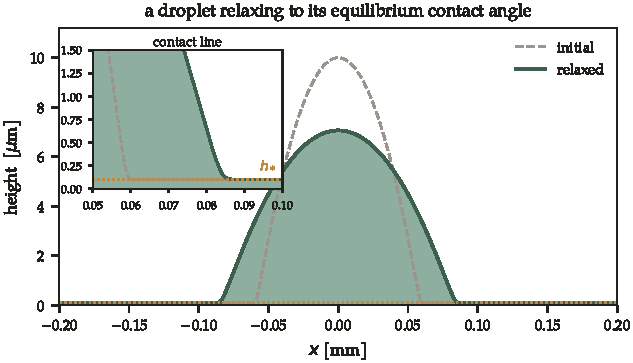
\includegraphics[width=0.85\textwidth]{../figures/wetting.pdf}
  \caption{平衡に向かう液滴（\file{wet\_static.toml}、$\thetae = \ang{10}$）。
    初期条件（破線）は\ang{20}の平衡液滴で、高さは\SI{10}{\micro\metre}、前駆膜は
    $\Hstar = 0.01$（\SI{0.1}{\micro\metre}、点線）である。格子幅は$\Delta x = \SI{0.2}{\micro\metre}$とした。
    実線は、計算が定常状態に達した\SI{2.92}{\second}での自由表面である。液滴は見かけの接触角
    \ang{9.71}まで濡れ広がった。$\thetae$より小さいのは、次節で述べる前駆膜による偏りのためである。
    液滴を囲む平坦な液膜は、$\Hstar$より\SI{0.5}{\percent}厚い値（\cref{eq:Hf-Hmax}の$\Hf$）に落ち着く。
    挿入図は接触線付近の拡大である。\label{fig:wetting:relax}}
\end{figure}

\section{見かけの接触角と前駆膜による偏り}
\label{sec:wetting:apparent}

前駆膜が\emph{有限の}厚さをもつモデルでは、$\Hmax/\Hstar$が大きくない限り、平衡液滴の角度は$\thetae$に
ならない。液滴の外側の分離圧が消える領域では、\cref{eq:eq-ode}は$H'' = K$に帰着し、形状は放物線になる。
この放物線を$H = 0$まで外挿したときの勾配が、実験で測定する角度に対応する。
これは閉じた形で書ける。

\begin{equation}\label{eq:theta-cap}
  \thetacap = \varepsilon\,\sqrt{-2 K \Hmax}
            = \thetae \left( 1 - \frac{\Hstar}{2\Hmax} \right).
\end{equation}

$\thetae = 10^\circ$、$(n,m) = (3,2)$について\cref{eq:theta-cap}を評価した値を、計算した形状が実際に
到達する最大勾配と並べて\Cref{tab:apparent-angle}に示す。

\begin{yzntable}{見かけの接触角と形状の最大勾配（$\thetae = 10^\circ$、$(n,m)=(3,2)$）\label{tab:apparent-angle}}{@{}d d d@{}}
\textsf{\bfseries $\Hmax/\Hstar$} & \textsf{\bfseries 見かけの接触角 [deg]} &
\textsf{\bfseries 形状の最大勾配 [deg]} \\ \midrule
2    & 7.5000 & 0.6320 \\
5    & 9.0000 & 3.6012 \\
10   & 9.5000 & 5.4236 \\
20   & 9.7500 & 6.7634 \\
50   & 9.9000 & 7.9627 \\
100  & 9.9500 & 8.5652 \\
1000 & 9.9950 & 9.5504 \\
\end{yzntable}

\begin{warn}[$\Hmax/\Hstar = 2$では指定した角度がどこにも現れない]
  表の一行目に注目されたい。液滴の厚さが前駆膜のわずか二倍だと、見かけの接触角は$7.50^\circ$、形状の
  最も急な点の傾きは$0.63^\circ$である。\key{ContactAngle}に書いた$10^\circ$は、測定値としても、
  勾配としても、漸近値としても、解のどこにも現れない。これは離散化誤差ではないので、格子をどう細かく
  しても解消しない。

  具体的には、\textbf{\SI{2}{\micro\metre}の前駆膜の上にある\SI{10}{\micro\metre}の液滴は、
  接触角を測定するケースとして妥当ではない。}計算で角度を求めたい場合は、比が大きくなるように
  ケースの寸法を決める。どれだけ大きくすべきかは\cref{tab:apparent-angle}で判断する。
\end{warn}

三列目は二列目よりはるかにゆっくり収束する。$\Hmax/\Hstar = 100$でも、形状の最も急な
勾配は$8.57^\circ$で、$10^\circ$に14 \%ほど届かない。一方、見かけの接触角はすでに0.5 \%以内に収まっている。
\textbf{放物線の外挿ではなく、計算した形状の勾配から角度を測るのであれば、さらにかなり厚い液滴が
必要になる。}\Cref{tab:apparent-angle}は
\code{tools/\bk make\_equilibrium\_1d.py --out /dev/null --sweep}で再現できる。
掃引ではファイルを書かないが、\code{--out}は必須の引数なので、捨てるための出力先を指定する。

\section{ケースの寸法決め}
\label{sec:wetting:sizing}

形状が前駆膜から液滴本体へと変化する長さは

\begin{equation}\label{eq:transition-length}
  \ell = \frac{\hstar}{\thetae},
\end{equation}

である。ただし$\thetae$はラジアンで表す。$\thetae = 10^\circ$、$\hstar = \SI{0.2}{\micro\metre}$
では$\ell = \SI{1.15}{\micro\metre}$となる。ここから二つの要件が導かれ、この二つで格子が決まる。

\begin{tip}[接触線のケースの二つの目安]
  \begin{itemize}
    \item \textbf{接触線を解像するには、$\Delta x \le \ell/5$を目安とする。}
      遷移領域を解像できていないと、接触線の移動速度も、接触線のなす角度も正しく得られない。
    \item \textbf{指定した角度を得るには、液滴の高さを前駆膜の厚さで割った比を$\Hmax/\Hstar \ge 50$とするのが
      目安である}。\cref{tab:apparent-angle}によれば、これで見かけの接触角の誤差は1 \%以内に
      収まる。比が10なら5 \%、比が5なら10 \%ずれる。
  \end{itemize}
  これらは目安であり、定理ではない。\cref{tab:apparent-angle}と遷移領域の幅から読み取った切りのよい数値で、
  出発点を示すにすぎず、解の収束を保証するものではない。
  収束は格子の細分化で確認すること（\cref{ch:convergence}）。
\end{tip}

具体例を示す。$h_0 = \SI{10}{\micro\metre}$、$\hstar = \SI{0.2}{\micro\metre}$
（\key{PrecursorRatio}は\val{0.02}）、$\thetae = 10^\circ$とし、幅\SI{600}{\micro\metre}の
計算領域を\key{Grid.Nx} $=$ \val{2000}で分割すると、$\Delta x = \SI{0.3}{\micro\metre}$となる。
膜厚の比はちょうど50なので、二つ目の目安はちょうど満たす。一つ目は満たさない。
$\ell/5 = \SI{0.23}{\micro\metre}$に対して、$\Delta x = \SI{0.3}{\micro\metre}$は$\ell/3.8$であり、
目安よりわずかに\emph{粗い}。このケースは目安の内側ではなく、ちょうど境界線上にある。
\file{docs/validation.md}でもそのように記述している。そこでの測定によれば、この解像度で、濡れ広がった液滴と
独立に構築した平衡液滴の見かけの接触角は\SI{0.02}{\percent}まで一致する。$\Delta x \approx \ell$となる
$\Delta x = \SI{1.2}{\micro\metre}$でも同様に一致する。濡れ広がりの過程も、細かい格子の結果と
\SI{0.06}{\percent}まで一致する（\cref{sec:verification:spreading}）。ただし、これは\ang{10}の液滴
一つという条件の緩いケースである。目安は出発点にすぎず、判断の決め手は細分化である。

二つの目安は互いに相反する。これが接触線の計算を高価にしている。$\Hmax/\Hstar$を大きくするには、
$\hstar$を下げるのが手っ取り早い。しかし\cref{eq:transition-length}により$\ell$も同じ割合で
短くなるので、必要な格子も同じ倍率で細かくなる。角度の精度を上げるにはセル数を増やすしかなく、
無償では得られない。濡れの計算のコストを決めるのは、たいてい物理ではなくこのトレードオフである。

最後に、もう一つ連成に注意しておく。ケースに蒸発も含まれる場合、$\hstar$は乾燥の挙動にも影響する。
\cref{sec:terms:evaporation}の前駆膜補正$f_h$は、前駆膜が乾ききって消えるのを防ぐためのもので、
$\Hstar$を用いて定義しているからである。接触角を調整するために前駆膜の厚さを変えると、蒸発モデルも
同時に変わる。
